\documentclass{beamer}
\usetheme{metropolis}
%\usepackage[backend=biber]{biblatex}
%\usepackage{booktabs} 
\usepackage{url}
\def\UrlBreaks{\do\/\do-}
\usepackage{amsfonts, amsmath, lmodern}
\usefonttheme{serif}
\usepackage{algorithm}
\usepackage{algorithmic}


%plots
\usepackage{tikz}
\usepackage{pgfplots}
\usepackage{pgfplotstable}
\pgfplotsset{compat=newest}
\usepackage{subcaption}
\usepackage{csvsimple}
%bibliography numbers
\setbeamertemplate{bibliography item}{\insertbiblabel}

\graphicspath{{./pictures}}
\setbeameroption{show notes} % comment out for the real presentation

\title{Fast Search of the Optimal Contraction Sequence in Tensor Networks}

\author{Max Koch, Christian Ortlepp}


\institute{Friedrich-Schiller-Universität Jena}

\date{20. Januar 2023}




\begin{document}

\begin{frame}
	\titlepage
  \end{frame}

\begin{frame}{Gliederung}
	\tableofcontents
\end{frame}

\section{Einführung und Zielsetzung}
\begin{frame}{Einführung}
	TBD
\end{frame}

\section{Tensor-Kontraktionen}
\subsection{Allgemeines}

\begin{frame}{Begriffseinführungen}
	\begin{columns}
		\begin{column}{0.5\textwidth}
			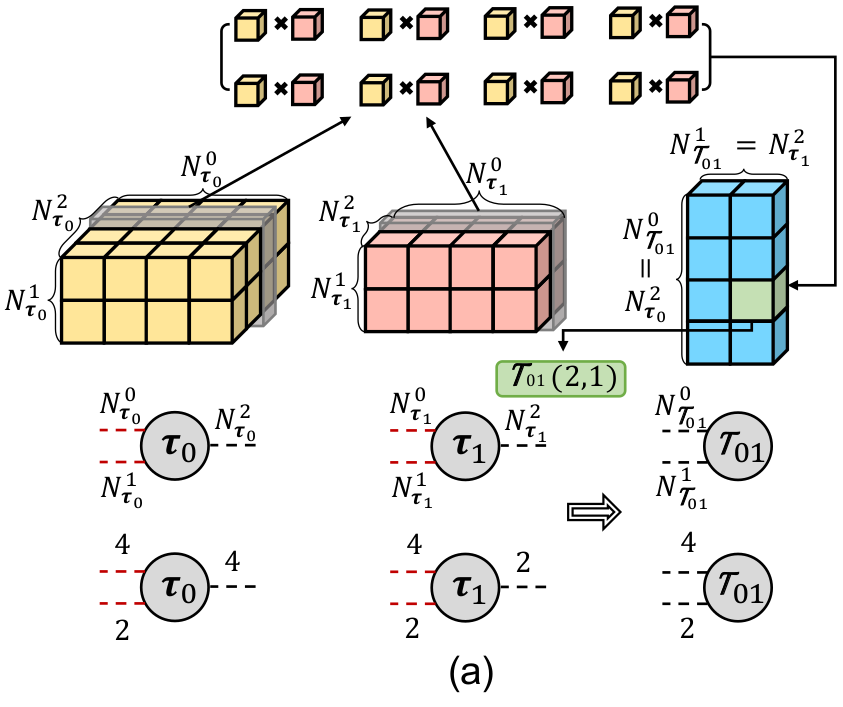
\includegraphics[scale=.2]{figure-2-a}
		\end{column}
		\begin{column}{0.5\textwidth}
			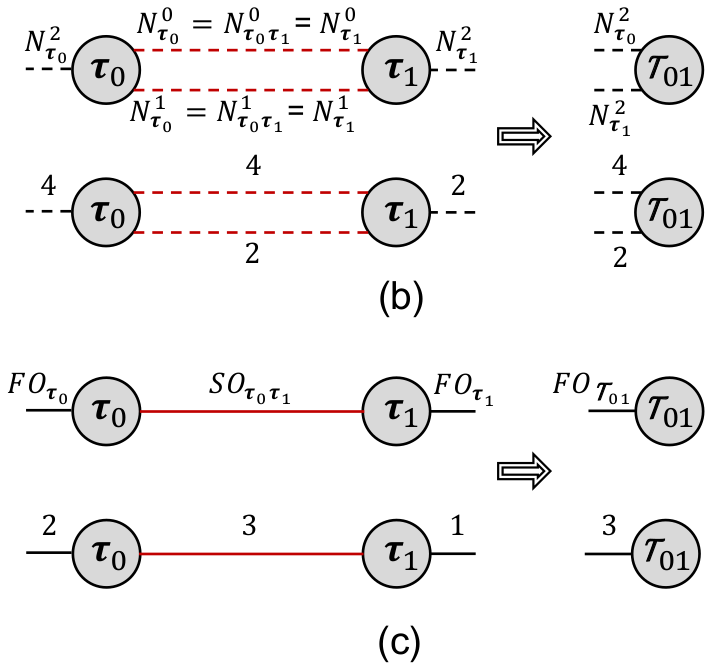
\includegraphics[scale=.2]{figure-2-b}
		\end{column}
	\end{columns}
\end{frame}
\note[itemize]{
\item Graph-Notation: Kanten=Dimensionen (Order), Knoten=Tensoren
\item Kanten zwischen Knoten "Sharing Orders", sonst "Free Orders"
\item Kantengewicht: $\log_2$ der Order
\item bei $V$ Tensoren werden $V-1$ Schritte benötigt
}

\begin{frame}{Kontraktion}
	\begin{columns}
		\begin{column}{0.5\textwidth}
			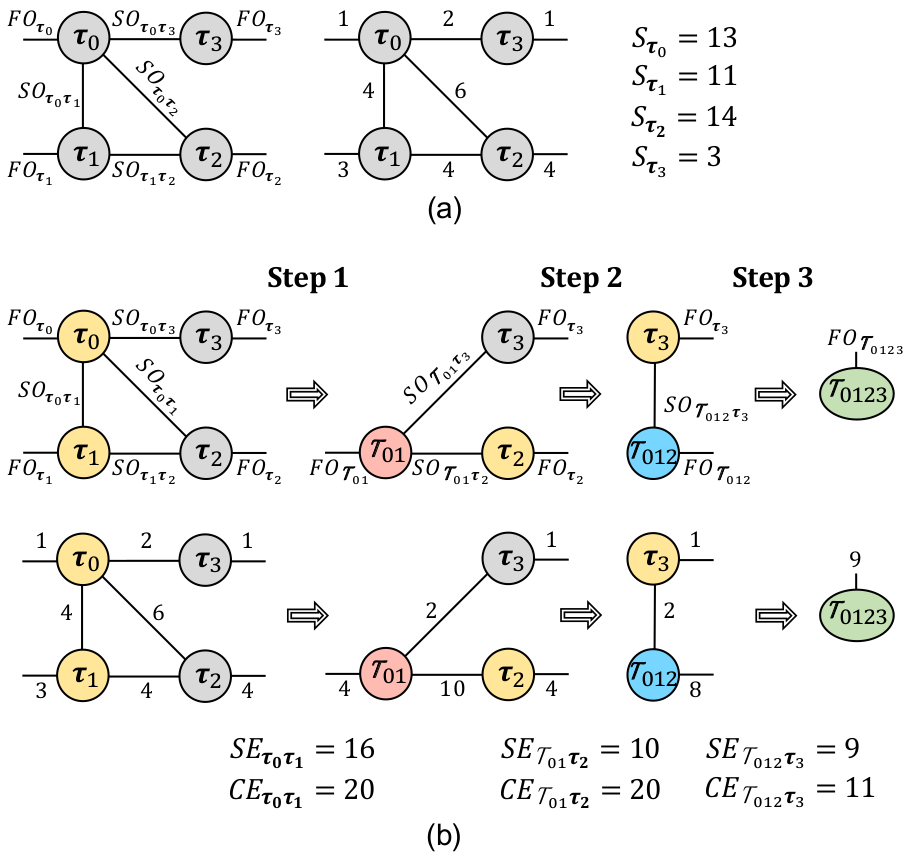
\includegraphics[scale=.17]{figure-3-a}
		\end{column}
		\begin{column}{0.5\textwidth}
			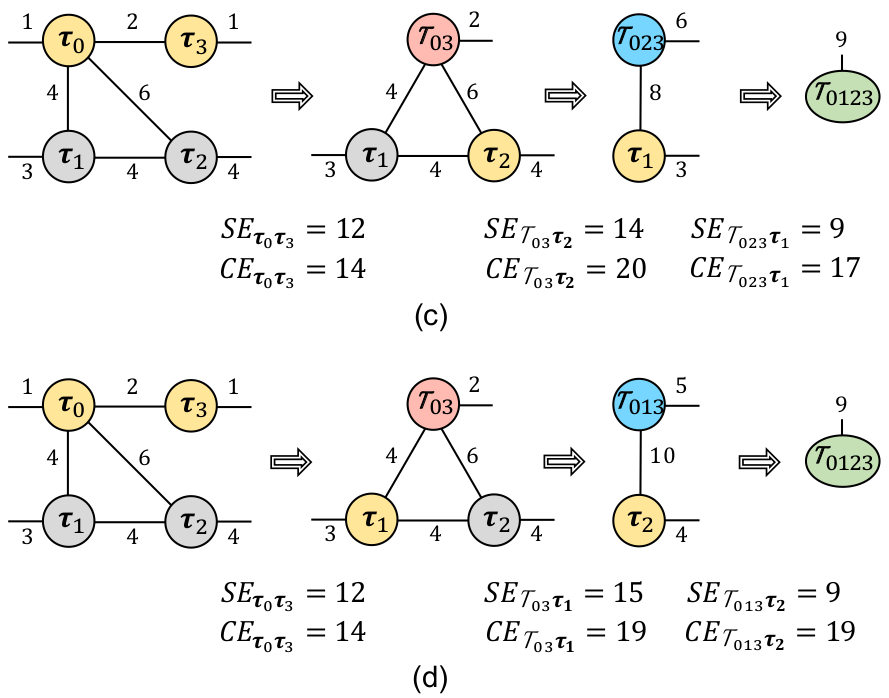
\includegraphics[scale=.17]{figure-3-b}
		\end{column}
	\end{columns}
\end{frame}
\note[itemize]{
\item verschiedene Kontraktionsreihenfolgen
\item bei jedem Schritt wird eine sharing order eliminiert
}

\subsection{BFS-Algorithmus}
\begin{frame}{BFS - Einführung}
	\begin{itemize}
		\item BFS = Breadth First Search
	\end{itemize}
\end{frame}
\note[itemize]{
	\item someNote
}


\section{Adjazenzmatrix-basierte Kontraktionssuche}


\subsection{Outer Product Pruning}
\begin{frame}{OPP - Einührung}
	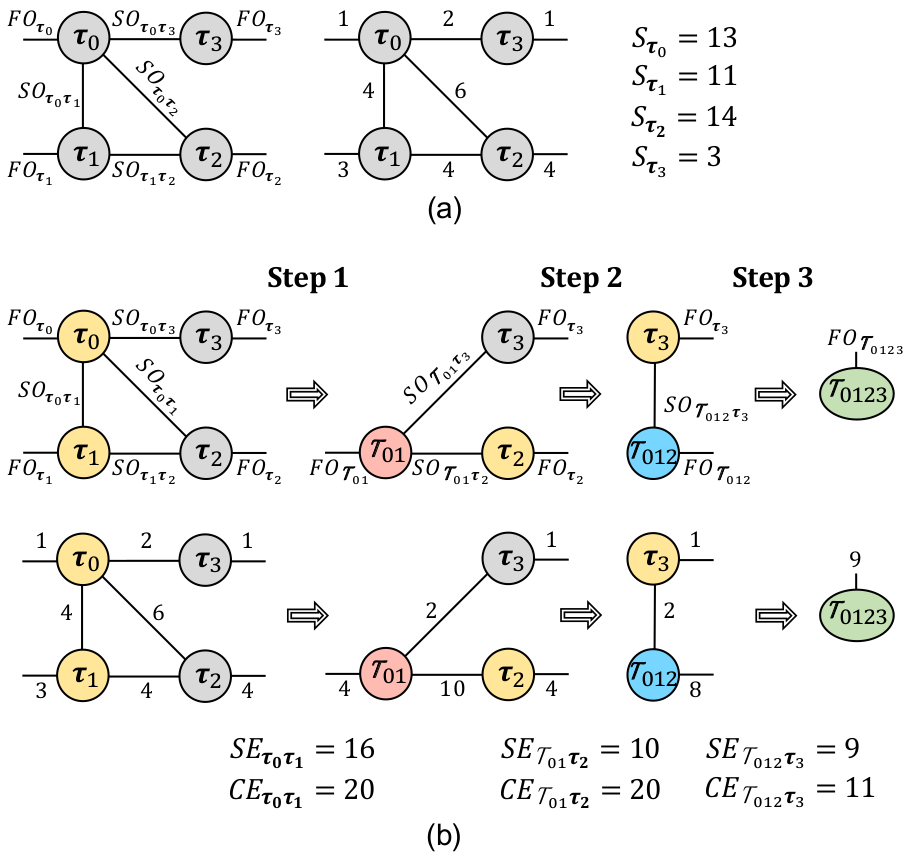
\includegraphics[scale=0.2]{figure-3-a}
\end{frame}
\note[itemize]{
	\item outer product: multiplikation von Tensoren ohne sharing Orders (siehe $\tau_2, \tau_3$)
	\item es ist bewiesen dass die beste Kontraktion (kleinste MS / MC) immer ohne outer - products auskommt
	\item[$\Rightarrow$] Outer products können bei Kontraktionen ausgeschlossen werden
	\item Wenn es im Netzwerk "Subnetzwerke" gibt, welche untereinander keine sharing orders teilen, kann in den subnetzwerken unabhängig voneinander nach der optimalen sequenz gesucht werden
}
\begin{frame}{OPP - Algorithmus}
	
\end{frame}
\note[itemize]{
	\item someNote
}




\begin{frame}[allowframebreaks]{Bibliography}
	\bibliography{../bibliography/bibliography.bib}
	\bibliographystyle{splncs04}
	\nocite{*}
\end{frame}

\end{document}
